\documentclass[12pt]{article}

\usepackage{lmodern}
\usepackage[T1]{fontenc}
\usepackage[utf8]{inputenc}
\usepackage[spanish, activeacute]{babel}
\usepackage{listings}
\usepackage{enumitem}
\usepackage{graphicx}
\usepackage{float}
\usepackage[hidelinks]{hyperref}

\usepackage{listings}
\usepackage{xcolor}

\definecolor{mygreen}{rgb}{0,0.6,0}
\definecolor{mygray}{rgb}{0.85,0.85,0.85}
\definecolor{mymauve}{rgb}{0.58,0,0.82}

\lstset{
  backgroundcolor=\color{mygray},   
  basicstyle=\ttfamily,        
  breakatwhitespace=false,         
  captionpos=b,                    
  commentstyle=\color{mygreen},    
  deletekeywords={...},            
  escapeinside={\%*}{*)},          
  extendedchars=true,              
  keepspaces=true,                 
  %keywordstyle=\color{blue},       
  language=Octave,                 
  morekeywords={require},            
  numbers=left,                    
  numbersep=5pt,                   
  numberstyle=\tiny\color{black}, 
  showspaces=false,                
  showstringspaces=false,          
  showtabs=false,                  
  stepnumber=1,                    
  stringstyle=\color{mymauve},     
  tabsize=2,                       
}

\graphicspath {{ assets/images/ }}

\title{BASES DE NODE.JS}
\author{ 
    Wilson Aguilar \\
    \textsc{Plataformas Web} 
}

\begin{document}

\maketitle

\section{Documentación}

\subsection{Requerir paquetes}

NodeJs tiene varias librerias o módulos que podemos utilizar que nos otorgan varias funcionalidades que pueden ser de ayuda en nuestro prógrama, ademas podemos instalar módulos adicionales por si necesitamos de alguna funcionalidad extra.

Para ello utilizamos la funcion \colorbox{mygray}{\lstinline{require(modulo)}} donde el modulo es el nombre del paquete que vamos a utilizar.

\begin{figure}[H]
    \centering
    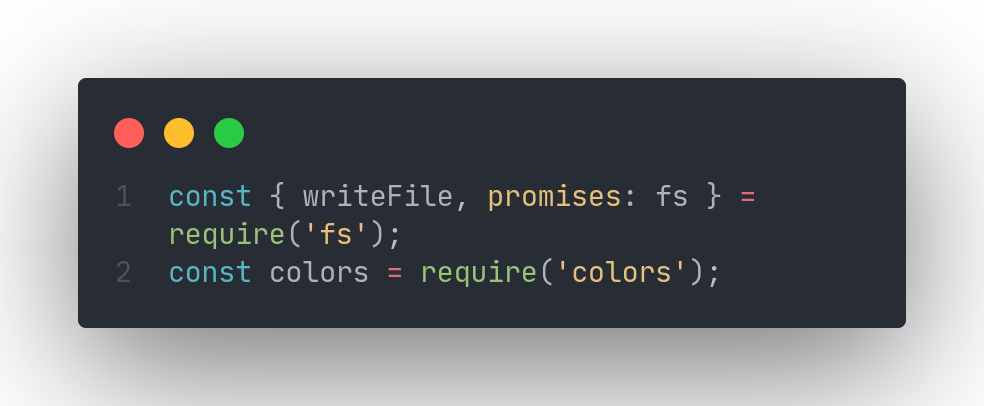
\includegraphics[scale=.3]{assets/images/require.png}
    \caption{require en NodeJs}
\end{figure}


\subsection{Importar archivos al proyecto}

A medida de que la aplicación que desarrollamos se va haciendo mas grande, es necesario dividir nuestro código en módulos para poder reutilizar partes del código que ya hayamos hecho. Por lo general un módulo esta conformado por varias funciones, para que estas funciones puedan ser accedidas desde otro archivo primero hay que exportarlas.

Utilizamos el objeto \colorbox{mygray}{\lstinline{module.exports}} que es un objeto de NodeJs que nos indica que funciones van a poder ser accedidas desde otro archivo.

\begin{figure}[H]
    \centering
    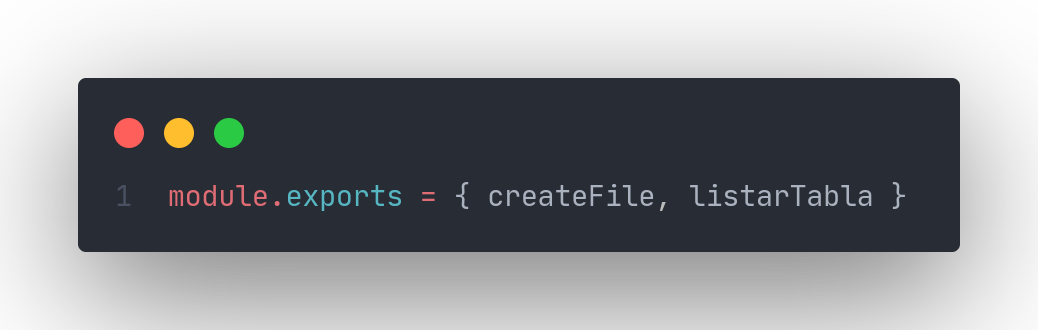
\includegraphics[scale=.25]{assets/images/export.png}
    \caption{export modules}

\end{figure}

\subsection{Recibir información de la línea
    de comandos}

La lógica principal de la aplicación se encuentra en el archivo app.js que es el encargado de recibir el comando que enviamos y en base a ese comando ejecutar alguna acción.

\begin{figure}[H]
    \centering
    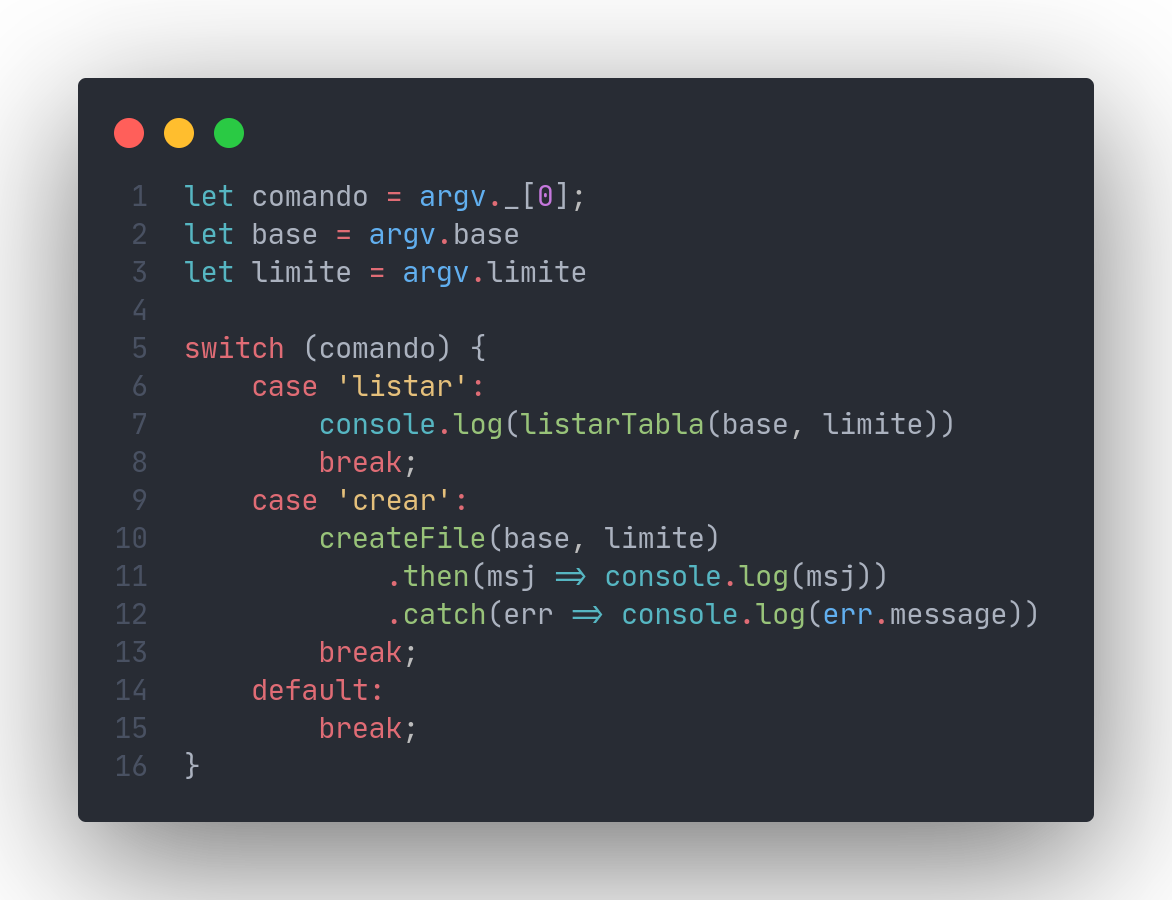
\includegraphics[scale=.25]{assets/images/app.png}
    \caption{app.js - Encargado de recibir los comandos}
\end{figure}

\subsection{Manejo de paquetes}

npm es una herramienta de NodeJs que nos ayuda a administrar nuestro proyecto y los módulos que vamos necesitando.

Para iniciar un nuevo proyecto de npm ejecutamos \colorbox{mygray}{\lstinline{npm init}}, despúes nos preguntará algunas opciones de nuestro proyecto y al final se creará un archivo llamado \lstinline{package.json} con la descripción de nuestro proyecto. Tambien podemos ejecutar \colorbox{mygray}{\lstinline{npm init -y}} si queremos saltarnos las preguntas.

Con el comando \colorbox{mygray}{\lstinline{npm install --save <nombre-paquete>}}, podremos agregar nuevos modulos que a nuestro proyecto.

Con el comando \colorbox{mygray}{\lstinline{npm install --save-dev <nombre-paquete>}} instalaremos el módulo como dependencia de desarrollo, esto nos indica que ese módulo no es necesario para que la aplicacion funcione, sino que ayuda al desarrollo de la misma.

Para eliminar un paquete usamos \colorbox{mygray}{\lstinline{npm uninstall <nombre-paquete>}}.

Cabe resaltar que cualquier modificación que hagamos con npm afectará al archivo package.json ya que ahi es donde se guarda toda la información de nuestro proyecto.

\subsection{Yargs}

Yargs es un módulo de npm que nos ayuda al desarrollo de aplicaciones de consola, nos ayuda a manejar de una forma mucho mas fácil los argumentos, opciones, comandos, entre otras opciones.

Para instalar yargs utilizamos el comando \colorbox{mygray}{\lstinline{npm install --save yargs}}

\subsection{Configuración YARGS}

Yargs tiene varias funciones que nos permiten agregar comandos, opciones y entre otras. Esto nos permite desarrlar aplicaciones de consola mucho mas fácil, sin tener que preocuparnos por las validaciones.

Para usar yargs usamos \lstinline{require('yargs')} y justo despues de eso podemos empezar a agregarle opciones. El resultado nos devuelve el objeto ya configurado donde solo debemos aplicar la lógica para cada comando.

La funcion \lstinline{command(comando, descripcion, opciones)} nos permite crear un nuevo comando y recibe como argumentos el nombre del comando, su descripcion y un objeto con las opciones que tendrá el comando.

\begin{figure}[H]
    \centering
    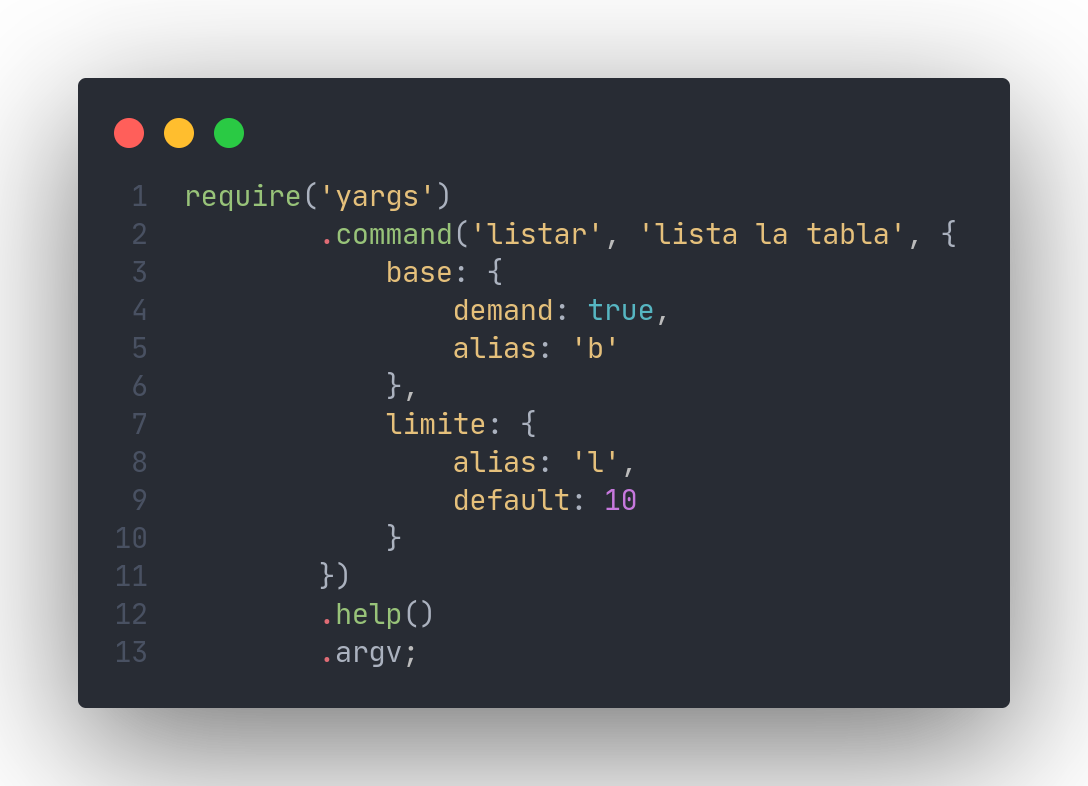
\includegraphics[scale=.3]{assets/images/yargs-config.png}
    \caption{Configuración básica de yargs}
\end{figure}

\subsection{Optimización de Yargs}

Para optimizar el código se movió toda la configuración de yargs a un archivo separado, creacion un objeto con las configuraciones para no tener que volver a escribir lo mismo y lo exportamos para que podamos usarlo en el archivo principal app.js

\begin{figure}[H]
    \centering
    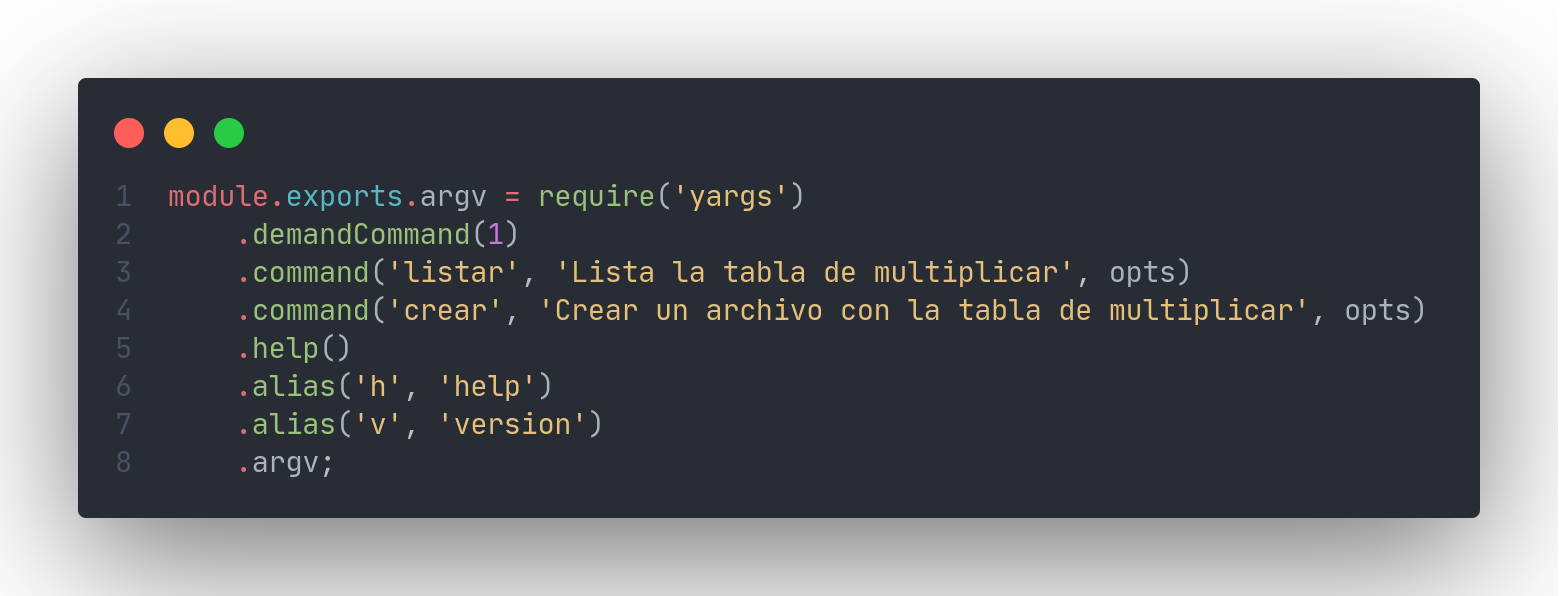
\includegraphics[scale=.24]{assets/images/yargs-opt.png}
    \caption{Optimización en yargs}
\end{figure}

\subsection{Colores en la Consola}

Para poder agregar colores a nuestra aplicacion instalamos el módulo colors de npm con \colorbox{mygray}{\lstinline{npm install --save colors}}.

Ahora para utilizarlo hacemos un \lstinline{require('colors')} en nuestro archivo mutiplicar.js, despues para agregar colores es tan facil como ejecutar un metodo en cualquier string como  \lstinline{"hola mundo".green}

\begin{figure}[H]
    \centering
    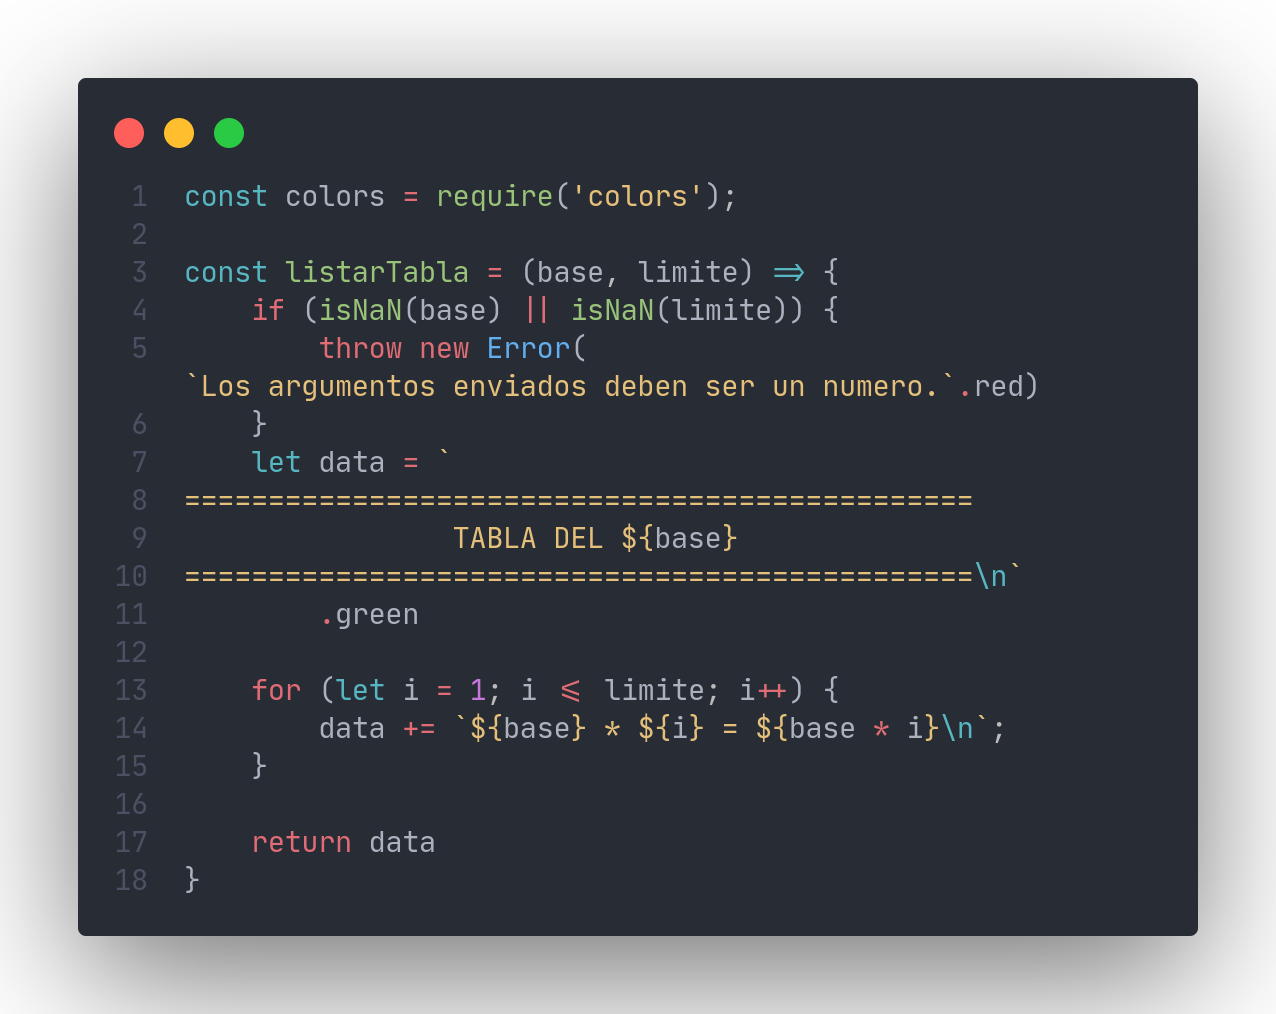
\includegraphics[scale=.3]{assets/images/colors.png}
    \caption{Uso colors}
\end{figure}

\newpage

\section{Github}

\subsection{Publicar proyecto en GitHub}

Para subir nuestro proyecto a github debemos crear uno vacio. Después lo agregamos como repositorio remoto con el commando

\lstinline{git remot add <nombre> <url>}

Una vez configurado el repositorio agregamos todos nuestros archivos con

\lstinline{git add -A}

Después hacemos un commit con:

\lstinline{git commit -m "primer commit"}

Por último subimos los cambios al repositorio remoto con el comando:

\lstinline{git push -u origin master}

\section{Repositorio}

El repositorio donde se encuentra el codigo es el siguiente:

\url{https://github.com/WilsonAG/plataformas-web.git}









\end{document}